\documentclass[aspectratio=169,xcolor=dvipsnames]{beamer}
\usepackage{hyperref}
\usepackage{graphicx, animate}
\usepackage{booktabs}
\usepackage{bbm} % indicatrices

\usetheme{SimpleDarkBlue}

\newcommand{\bdOne}{\mathbbm{1}}

\title{Stratification: Monte Carlo and Simulation}
\author{
    Alban \textsc{Géron}, \\
    Arnaud \textsc{Barrat}, \\
    Camille \textsc{Legrée-Hagbarth}, \\
    Tristan \textsc{Fabre}
}
\date{April 29\textsuperscript{th}, 2025}



\begin{document}
    \begin{frame}
        \titlepage
    \end{frame}

    \begin{frame}{Introduction}
        % @Arnaud ? jsp trop ce que tu voulais mettre pour le benchmark
    \end{frame}

    \begin{frame}{Problem}
        We aim to estimate the integral
        %
        \[I = \int_{[0, 1]^d} f(u) du\]
        %
        where, for all $u = (u_1, \dots, u_d) \in [0, 1]^d$,
        %
        \[f(u) = \cos\left(2 \pi \left(\frac{1}{d} \sum_{i = 1}^d u_i - \frac{1}{2}\right)\right)\]
    \end{frame}

    \begin{frame}{Summary}
        \tableofcontents
    \end{frame}

    \section{Estimation methods used to solve the problem (Monte-Carlo, quasi-Monte-Carlo)}

    \begin{frame}{Monte-Carlo}
        \begin{itemize}
            \item<1-> Notice that $I = \mathbb{E}[f(U)]$, where $U \sim \mathcal{U}([0, 1]^d)$.

            \item<2-> Thus, following Monte-Carlo's method, we approximate such an expectation by
            %
            \[\frac{1}{N} \sum_{n = 1}^N f(U_n)\]
            %
            where $N$ is a large integer and the $U_n$'s are $N$ i.i.d. random vectors uniformly distributed on $[0, 1]^d$.
        \end{itemize}
    \end{frame}

    \begin{frame}{Quasi-Monte-Carlo}
        \begin{itemize}
            \item<1-> In the course's slides, quasi-Monte-Carlo has been proven to be more efficient in terms of computation than Monte-Carlo, under weak assumptions.

            \item<2-> Again, we approximate $I = \mathbb{E}[f(U)]$ by the empirical mean $\frac{1}{N} \sum_{n = 1}^N f(U_n)$, but here the $U_n$'s are generated in the set $\mathcal G = \left\{\frac{1}{2N}, \frac{3}{2N}, \dots, \frac{2N - 1}{2N}\right\}^d$ under the condition \eqref{eq:cdC}:
            %
            \begin{equation}
                \alert{\text{each one of the points } U_1, \dots, U_N \text{ falls on exactly one strip of the set } \mathcal G} \tag{C}\label{eq:cdC}
            \end{equation}

            \item<3-> For $d = 2$: the condition \eqref{eq:cdC} means that there is exactly one point in each line and each column:
            %
            \begin{center}
                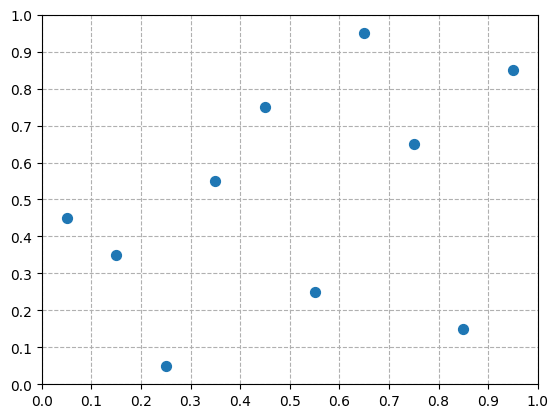
\includegraphics[width=\textwidth/3]{points2.png}
            \end{center}
        \end{itemize}
    \end{frame}

    \begin{frame}{Quasi-Monte-Carlo}
        \begin{itemize}
            \item For $d = 3$:
            %
            \begin{center}
                \animategraphics[autoplay,loop,width=0.6\linewidth]{10}{gif_frames/frame_}{000}{179}
            \end{center}
        \end{itemize}
    \end{frame}

    \begin{frame}{Quasi-Monte-Carlo}
        \begin{itemize}
            \item \eqref{eq:cdC} boils down to generating a $d$-dimensional table $M = (m_{i_1, \dots, i_d}) \in \mathbb{R}^{N^d}$ such that
            %
            \[m_{i_1, \dots, i_d} = \bdOne_{i_1 = \sigma_2(i_2) = \cdots = \sigma_d(i_d)}, \qquad \forall (i_1, \dots, i_d) \in \{0, 1, \dots, N - 1\}^d\]
            %
            where $\sigma_2, \dots, \sigma_d$ are $d - 1$ permutations of $\{0, 1, \dots, N - 1\}$, generated independently and uniformly on the (finite) set of permutations $\mathfrak{S}(\{0, 1, \dots, N - 1\})$.
        \end{itemize}
    \end{frame}

    \section{Implementation of unbiased estimators using N. \textsc{Chopin}'s paper}

    \begin{frame}{Frame Title}
        
    \end{frame}

    \section{Implementation of importance sampling methods}

    \begin{frame}{Frame Title}
        
    \end{frame}
\end{document}